\section{ШИМ управление с использование ПИД регулятора}\label{sec:ch3/sec2}

\subsection{Принципы реализации ШИМ в пневматических системах с дискретным управлением}\label{subsec:ch3/sec2/sub1}
Широтно-импульсная модуляция (ШИМ) представляет собой метод формирования квазинепрерывного
управляющего воздействия в системах с дискретными исполнительными элементами.
В контексте пневматических систем с дискретными распределителями применение ШИМ
позволяет преодолеть ограничения, связанные с бинарным характером управления, и обеспечить более
точное регулирование положения и скорости исполнительного механизма.

Механизм формирования квазинепрерывного управляющего воздействия
посредством ШИМ основан на периодическом переключении дискретных
распределителей с определенной частотой и скважностью.

Математически это может быть описано следующим образом:

\begin{equation}
	u(t) = \begin{cases}
		1, & 0 \leq t < \alpha T \\
		0, & \alpha T \leq t < T
	\end{cases}
\end{equation}
где $u(t)$ -- управляющий сигнал;
$T$ -- период ШИМ;
$\alpha$ -- коэффициент заполнения $0 \leq \alpha \leq 1$.

На рисунке \ref{fig:ch3:pwm_example} показаны временные диаграммы ШИМ-сигнала
с различными значениями коэффициента заполнения.

\begin{figure}[ht]
	\centerfloat{
		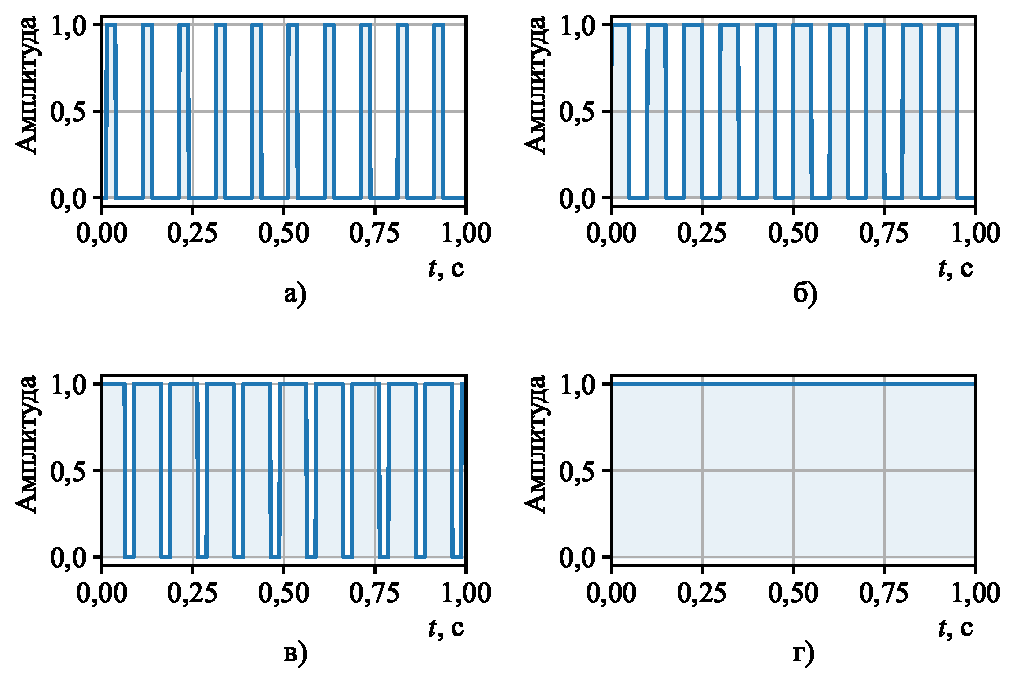
\includegraphics[]{part3/pwm_signal_skewness.pdf}
	}
	\caption{Примеры ШИМ-сигнала с различными значениями коэффициента заполнения:\\ а) $\alpha = \num{0.3}$; б) $\alpha = \num{0.6}$; в) $\alpha = \num{0.9}$}
	\label{fig:ch3:pwm_example}
\end{figure}

Среднее значение управляющего воздействия за период определяется как:
\begin{equation}
	\bar{u} = \frac{1}{T} \int_0^T u(t) dt = \alpha,
\end{equation}

Влияние частоты ШИМ на динамику пневмопривода является критическим фактором при
проектировании системы управления. С увеличением частоты ШИМ улучшается
гладкость управляющего воздействия, что способствует снижению пульсаций давления
и повышению точности позиционирования. Однако чрезмерно высокая частота может привести
к повышенному износу распределителей и увеличению энергопотребления.

Для анализа влияния частоты ШИМ на динамику системы может быть использована передаточная функция эквивалентного непрерывного звена:
\begin{equation}
	W_{\text{ШИМ}}(s) = \frac{1 - e^{-sT}}{sT},
\end{equation}
где $s$ -- комплексная переменная преобразования Лапласа.
Особенности применения ШИМ для различных типов дискретных
распределителей обусловлены их конструктивными характеристиками и
динамическими свойствами. На рисунке \ref{fig:ch3:pwm_valve_response} показаны
характеристики переходных процессов для распределителя с временем срабатывания $\tau = 30$~мс и различной
частотой ШИМ сигнала.

\begin{figure}[ht]
	\centering
	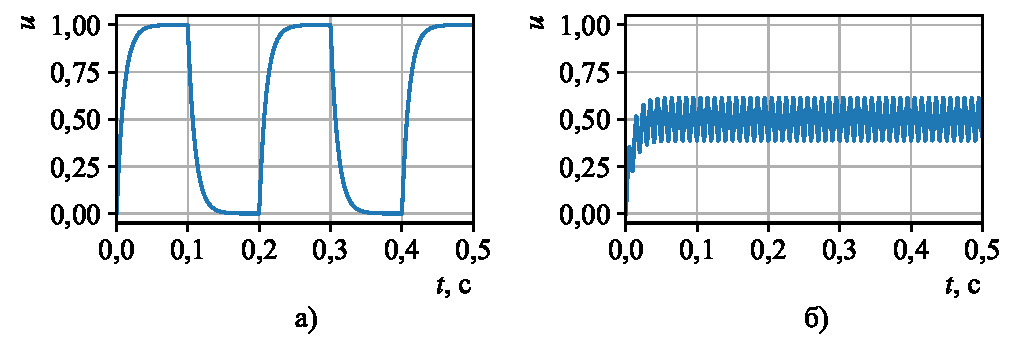
\includegraphics[]{part3/pwm_signal_transfer_function.pdf}
	\caption{Характеристики переходных процессов при различной частоте ШИМ:\\
		а) $f_{\text{ШИМ}} = \num{5}$~Гц; б) $f_{\text{ШИМ}} = \num{100}$~Гц
	}
	\label{fig:ch3:pwm_valve_response}
\end{figure}

При выборе параметров ШИМ необходимо учитывать соотношение между
периодом ШИМ и динамическими характеристиками распределителя:
\begin{equation}
	T_{ШИМ} \geq k\tau_{\text{р}},
\end{equation}
где $\tau_{\text{р}}$ -- время реакции распределителя;
$k$ -- коэффициент запаса (обычно $k \geq 2$).

\subsection{Реализация ПИД-регулирования для пневмоприводов с дискретными распределителями}\label{subsec:ch3/sec2/sub2}

Применение ШИМ в пневмоприводах с дискретными распределителями открывает
возможность использования алгоритмов управления,
изначально разработанных для непрерывных систем.
Одним из наиболее эффективных и широко применяемых методов является
пропорционально-интегрально-дифференциальное (ПИД) регулирование.

Структура ПИД-регулятора для пневмопривода
с дискретными распределителями представлена на рисунке \ref{fig:ch3:pid_pwm_control}.

\begin{figure}[ht]
	\centering
	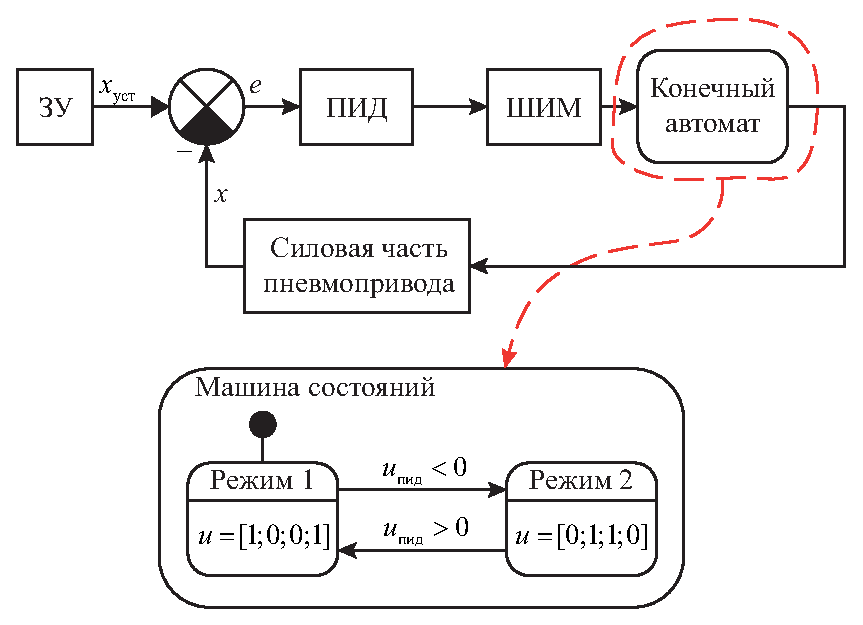
\includegraphics[]{part3/pid_pwm.eps}
	\caption{Структурная схема ПИД-регулятора с ШИМ управлением}
	\label{fig:ch3:pid_pwm_control}
\end{figure}

В данной схеме выходной сигнал ПИД-регулятора преобразуется в коэффициент
заполнения ШИМ, который управляет дискретными распределителями
пневмопривода. Этот подход позволяет достичь высокой точности
управления, характерной для непрерывных систем, в условиях
дискретного исполнительного механизма.

Математическая модель ПИД-регулятора в непрерывной форме описывается уравнением:
\begin{equation}\label{eq:pid_base}
	u_{\text{пид}}(t) = K_{\text{п}} e(t) + K_{\text{и}} \int_0^t e(\tau)d\tau + K_{\text{д}}\frac{de(t)}{dt},
\end{equation}
где
$e(t)$ -- ошибка регулирования;
$K_\text{п}$, $K_\text{и}$, $K_\text{д}$ -- коэффициенты пропорциональной, интегральной и
дифференциальной составляющих соответственно;

Выходной сигнал ПИД-регулятора преобразуется в коэффициент заполнения ШИМ согласно формуле:
\begin{equation}
	\alpha = \frac{u(i) + u_{max}}{2u_{max}},
\end{equation}
где $u_{max}$ -- максимальное значение управляющего сигнала.

Однако в рассматриваемой конфигурации ПП с дискретными распределителями
выходной сигнал ПИД-регулятора, как сказано выше, преобразутеся в бинарное
управляющее воздействие посредством ШИМ. При этом возможна только реализация
только двух основных режимов движения: выдвижение штока и его втягивание.

Математически это может быть описано следующим образом:

\begin{equation}
	\mathbf{u}(t) = \begin{cases}
		[1,0,0,1], & \text{если } u_\text{пид}(t) > 0 \\
		[0,1,1,0], & \text{если } u_\text{пид}(t) < 0
	\end{cases}
\end{equation}
где $u_\text{пид}(t)$ -- выходной сигнал ПИД-регулятора.

Существенным ограничением данного подхода является отсутствие
прямого управления режимом торможения привода, что может приводить к
перерегулированию и колебательности системы. Выходной сигнал ПИД-регулятора
преобразуется в коэффициент заполнения ШИМ согласно формуле:

\begin{equation}
	\alpha = \begin{cases}
		\frac{u_\text{ПИД}(t)}{u_{max}},  & \text{если } u_\text{ПИД}(t) > 0 \\
		-\frac{u_\text{ПИД}(t)}{u_{max}}, & \text{если } u_\text{ПИД}(t) < 0
	\end{cases}
\end{equation}
где $u_{max}$ -- максимальное значение управляющего сигнала.

Данное ограничение является одной из ключевых причин для рассмотрения модифицированных
структур управления, способных обеспечить более эффективное торможение и позиционирование
привода за счет использования дополнительных режимов работы распределителей или реализации
торможения.

\subsection{Модифицированная структура ПИД-регулятора}\label{subsec:ch3/sec2/sub3}

Как было написано выше классическая структура ПИД-регулятора с ШИМ управлением имеет существенные ограничения
в обеспечении эффективного управления электропневматическим приводом с дискретными распределителями.
Основным недостатком является отсутствие прямого управления режимом торможения, что приводит к значительному
перерегулированию и колебательности системы. Для преодоления данных ограничений предлагается модифицированная
структура ПИД-регулятора, обеспечивающая адаптивное торможение на основе анализа динамического состояния системы.

Предложенная модификация базируется на концепции прогнозирования тормозного пути и формировании упреждающего
управляющего воздействия. Математическая модель модифицированного ПИД-регулятора включает три основных
компонента: классический ПИД-регулятор описанный выражением \ref{eq:pid_base}, блок прогнозирования тормозного пути
и блок формирования тормозного воздействия.

Прогнозирование тормозного пути осуществляется на основе анализа
кинетической энергии системы и желаемого ускорения торможения:
\begin{equation}\label{eq:braking_prediction}
	s_{\text{торм}}(t) = \frac{v(t)|v(t)|}{2a_{\text{торм}}} + \frac{K_{\text{б}}v(t)^2}{2}\text{,}
\end{equation}
где $v(t)$ -- текущая скорость привода;
$a_{\text{торм}}$ -- желаемое ускорение торможения;
$K_{\text{б}}$ -- коэффициент запаса по тормозному пути, учитывающий инерционность пневматической системы.

Эффективность торможения определяется соотношением между прогнозируемым тормозным путем
и расстоянием до целевой точки. Коэффициент интенсивности торможения вычисляется с использованием нелинейной функции:
\begin{equation}\label{eq:braking_intensity_expanded}
	k_{\text{торм}}(t) = \begin{cases}
		\left(1 - \min\left(\frac{s_{\text{цель}}(t)}{s_{\text{торм}}(t) \cdot k_{\text{порог}}}, 1\right)\right)^2 \cdot \eta(v), & |v(t)| > v_{\text{порог}}    \\
		0,                                                                                                                         & |v(t)| \leq v_{\text{порог}}
	\end{cases}
\end{equation}
где $s_{\text{цель}}(t) = |x_{\text{зад}} - x(t)|$ -- расстояние до целевой точки;
$k_{\text{порог}}$ -- пороговый коэффициент начала торможения;
$\eta(v)$ -- функция модуляции интенсивности торможения:
\begin{equation}\label{eq:modulation_function}
	\eta(v) = 1 - \exp\left(-\left(\frac{|v(t)|}{v_{\text{хар}}}\right)^2\right)\text{,}
\end{equation}
где $v_{\text{хар}}$ -- характерная скорость, определяющая форму функции модуляции.

Результирующее управляющее воздействие формируется путем комбинации сигналов ПИД-регулятора и тормозного контура:
\begin{equation}\label{eq:combined_control}
	u_{\text{м}}(t) = (1 - k_{\text{торм}}(t))u_{\text{пид}}(t) + k_{\text{торм}}(t)u_{\text{торм}}(t)\text{,}
\end{equation}
где $u_{\text{торм}}(t)$ -- сигнал управления в режиме торможения, определяемый направлением движения:
\begin{equation}\label{eq:braking_control_expanded}
	\mathbf{u}_{\text{торм}}(t) = \begin{cases}
		[0, \alpha{\text{т}}(t), \alpha_{\text{т}}(t), 0],  & v(t) > v_{\text{порог}}      \\
		[\alpha_{\text{т}}(t), 0, 0, \alpha_{\text{т}}(t)], & v(t) < -v_{\text{порог}}     \\
		[0, 0, 0, 0],                                       & |v(t)| \leq v_{\text{порог}}
	\end{cases}
\end{equation}

Коэффициент заполнения ШИМ в режиме торможения вычисляется с учетом динамических характеристик системы:
\begin{equation}\label{eq:braking_pwm_expanded}
	\alpha_{\text{т}}(t) = k_{\text{торм}}(t) \cdot \alpha_{\text{макс}} \cdot \left(1 + K_{\text{к}}\frac{d|v(t)|}{dt}\right),
\end{equation}
где $K_{\text{к}}$ -- коэффициент коррекции, учитывающий скорость изменения модуля скорости.

Для обеспечения численной устойчивости и плавности переключения режимов вводится гистерезисная характеристика активации торможения:
\begin{equation}\label{eq:hysteresis}
	v_{\text{порог}}(t) = v_{\text{порог}}^0 \cdot \begin{cases}
		1 + \Delta v, & \text{при переходе к торможению} \\
		1 - \Delta v, & \text{при выходе из торможения}
	\end{cases}
\end{equation}
где $v_{\text{порог}}^0$ -- базовое пороговое значение скорости;
$\Delta v$ -- ширина гистерезиса.

Исследование динамических характеристик системы управления электропневматическим приводом демонстрирует существенные различия
в характере переходных процессов для классической и модифицированной структур ПИД-регулятора с ШИМ.

Для классической структуры характерно наличие значительной колебательности, обусловленной отсутствием эффективного
управления торможением. Это проявляется в перерегулировании при подходе к заданной позиции и возникновении
затухающих колебаний из-за ограниченности режимов работы распределителей.


Модифицированная структура обеспечивает более качественный переходный процесс благодаря
адаптивному торможению и прогнозированию тормозного пути. Показатели качества позиционирования
предвставлены в таблице \ref{tab:system_params_pid}.

\begin{figure}[ht!]
	\centerfloat{
		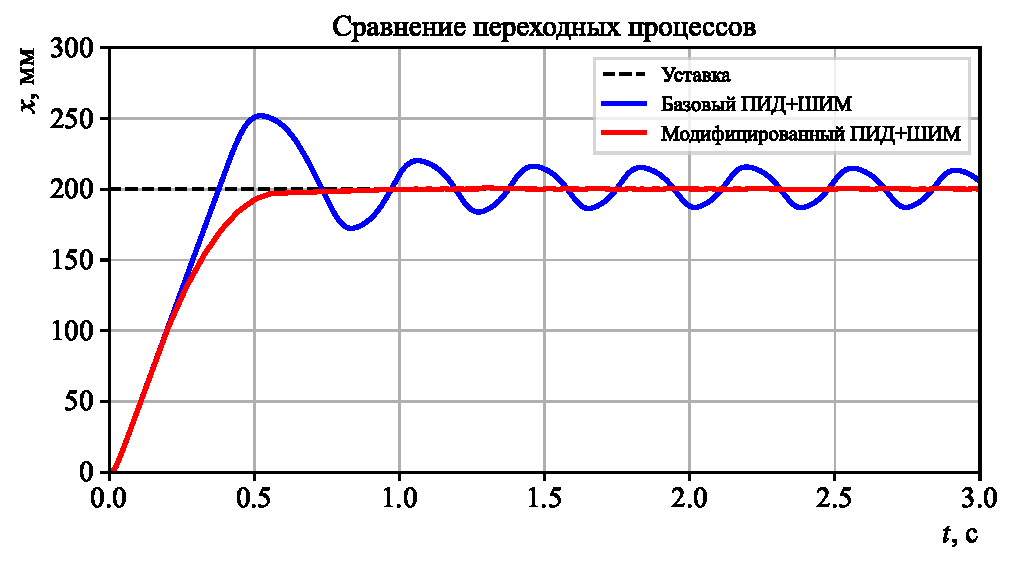
\includegraphics[]{part3/pid_comparison.pdf}
	}
	\caption{Сравнение переходных процессов для классической и модифицированной структуры ПИД-регулятора с ШИМ}
	\label{fig:ch3:transient_comparison}
\end{figure}

\begin{table}[h!]
	\centering
	\caption{Показатели качества позиционирования для модифицированной структуры ПИД-регулятора с ШИМ}
	\small
	\begin{tabular}{lccl}
		\textbf{Показатель качества}            & \textbf{Обозначение}   & \textbf{Значение} & \textbf{Размерность} \\
		\midrule
		Время переходного процесса              & $t_\text{п}$                  & \num{0.39}        & с                    \\
		Перерегулирование                       & $\sigma$               & \num{0}           & \%                   \\
		Статическая ошибка                      & $|\Delta_{\text{ст}}|$ & \num{1.31}        & мм                   \\
		Среднее количество переключений за цикл & $N_\text{п}$           & 57                & -                    \\
		\midrule
	\end{tabular}
	\label{tab:system_params_pid}
\end{table}

Представленные на рисунке \ref{fig:ch3:transient_comparison} результаты наглядно демонстрируют
преимущества модифицированной структуры в обеспечении качества позиционирования электропневматического привода.